\documentclass[a4paper]{article}
\usepackage{graphicx}
\usepackage[margin = 1in]{geometry}
\usepackage{ragged2e}
\usepackage[normalem]{ulem}
\usepackage[hidelinks, colorlinks = true, citecolor = black, linkcolor = blue]{hyperref}
\usepackage{parskip}
\usepackage{cite}
\usepackage{caption}
\usepackage{subcaption}
\usepackage{cellspace}
\usepackage{makecell}
\usepackage{mwe}
\setlength\cellspacetoplimit{4pt}
\setlength\cellspacebottomlimit{4pt}
\usepackage{caption} 
\usepackage{pgfplots}
\usepackage{amsmath}
\usepackage{tikz}
\usepackage{pdfpages}
\usetikzlibrary{tikzmark}
\newcommand{\inv}{^{\raisebox{.2ex}{$\scriptscriptstyle-1$}}}
\newcommand{\unit}[1]{~\mathrm{#1}}
\captionsetup[table]{skip=10pt}
\renewcommand{\arraystretch}{1.5}
\pgfplotsset{compat=1.16}
\pgfplotsset{ignore zero/.style={%
  #1ticklabel={\ifdim\tick pt=0pt \else\pgfmathprintnumber{\tick}\fi}
}}

\begin{document}
\section{Introduction}
DC power sources are an essential part of circuits. The aim of the following
experiments is to study the proprieties of these sources. Electromotive force,
ideal-source current, open-circuit voltage, short-circuit current, and internal
resistance will be studied for voltage sources.

The behaviour of series and parallel source arrangements will also be studied.

\section{Background/ Theory}
DC power sources refer to either voltage or current sources of which the output
does not diminish with time. A source is called an ideal voltage source when the
output voltage does not change in relation to the load resistance. For current
sources, the current remains constant regardless of the load resistor. 

In physical applications however, the current or voltage will depend on the load
resistance. Therefore, power sources will be represented as a combination
between an ideal source and an internal resistance. For voltage sources, the
resistance will be connected in series with the ideal source, whereas for
current sources, the resistor will be connected in parallel. (book)

Figures 1(a) and 1(b) display the aforementioned representation of power
sources, both for current and voltage sources.(lab text)

\begin{figure}[!ht]
    \centering
    \begin{subfigure}{0.5\textwidth}
        \centering
        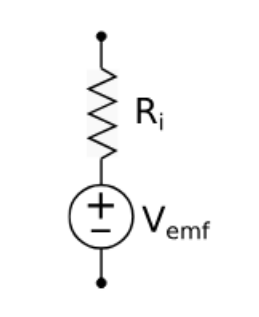
\includegraphics[width = 0.5 \linewidth]{Voltagesource.png}
    \label{fig:1a}
        \caption{Schematic representation of voltage source}
    \end{subfigure}%
    \begin{subfigure}{0.5\textwidth}
        \centering
        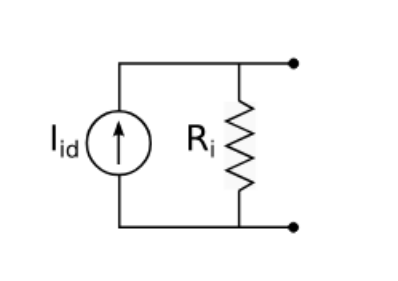
\includegraphics[width = 0.7\linewidth]{Currentsource.png}        
    \label{fig:1b}
        \caption{Schematic representation of current source}
    \end{subfigure}
\label{fig:1}
    \caption{Schematic representation of power sources}  
\end{figure}

\subsection{Source characteristics}
Using source transformation, all power sources can be represented as voltage
sources with an internal resistance(book). Therefore, going forward, sources
will be displayed as shown in Figure 1(a). This representation is called the
voltage-equivalent circuit. By adding a load resistance to the power source, essential characteristics of
the source can be discovered.

\newpage
Figure 2 displays the circuit which will be used to determine these
characteristics(labtext).

\begin{figure}[!ht]
    \centering
    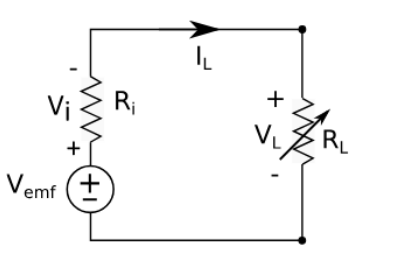
\includegraphics[width = 0.5\textwidth]{loadcircuit.png}
    \label{fig:2}
    \caption{Simple load circuit of real voltage source}
\end{figure}

Firstly, the voltage of the ideal source is called the electromotive force,
$V_{emf}$. By measuring the load current, this voltage can be related to the
load voltage by observing that the same current passes through the internal
resistance as well. 

Equation 1 displays the relationship between current, load
voltage, and electromotive force(labtext).

\begin{equation}
    V_L = V_{emf} + I_L R_i
\end{equation}

Since the internal resistance, $R_i$, is constant, the relationship between load
voltage and current is a linear one. 

Figure 3 displays this relationship for a
real voltage source such as the one shown in Figure 1(a)(labtext).

\begin{figure}[!ht]
    \centering
    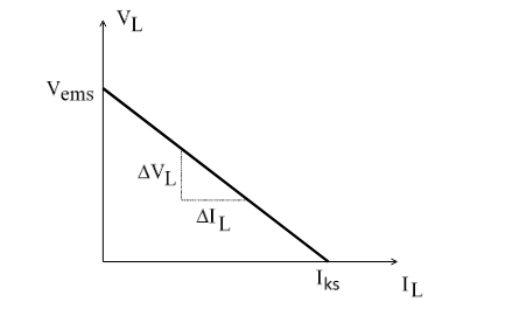
\includegraphics[width = 0.5\textwidth]{vi_graph.png}
    \label{fig:3}
    \caption{Typical $V_L$ - $I_L$ graph used to determine source characteristics}
\end{figure}

By determining the slope of the linear relationship between $I_L$ and $V_L$, the
internal resistance can be found(labtext):

\begin{equation}
    R_i = -\frac{\Delta V_L}{\Delta I_L}
\end{equation}

By looking at the x and y intercepts of the graph, both the electromotive force
and the short circuit current can be found. Therefore, all of the sources
characteristics can be found by analyzing the Voltage-Current graph.

A relationship between all of the characteristics is found equation 3(labtext):

\begin{equation}
    I_{sc} = \frac{V_{emf}}{R_i}
\end{equation}

\subsection{Series and parallel sources}
By connecting multiple voltage sources in series, higher $V_{emf}$ values can be
provided. The equivalent internal resistance will be equal to the sum of the
individual sources internal resistances.

When connecting multiple sources in parallel, the equivalent internal resistance
will be lowered. The lowering of the internal resistance will be governed by the
parallel resistance equivalence(labtext):

\begin{equation}
    R_i = \left( \sum_{j} \frac{1}{R_{i,~j}}\right) \inv
\end{equation}

Since sources should only be connected in parallel when they have the same
electromotive force, the equivalent $V_{emf}$ will be equal to that of one
source(labtext).

\subsection{Maximum power transfer}

When connection a load resistor in series with a voltage source, the
relationship between dissipated power and load resistance and load voltage is
governed by the following equation:

\begin{equation}
    P_L = \frac{V_l ^2}{R_l}
\end{equation}

However, since the power is also dissipated on the internal resistance, this
simple equation cannot be easily used to determine the maximum power transfer. If the
source was an ideal one, the power output would reach its maximum when $R_L \rightarrow
0$. Therefore, since both the internal resistance and the load resistor
contribute to power transfer, the maximal point will occur when:
\begin{equation}
    R_L = R_i
\end{equation}

Even so, it is important to mention that, since the power dissipated through the
load resistor will be equal to the power on the internal resistance, the
efficiency of the circuit will only reach $50\%$.(labtext)
\section{Method and materials}
We assembled all of the circuits using the provided circuit building system. We
measured everything, including voltage and current, using an AM-520
HVAC mutlimeter. 1.5 V batteries were used as voltage sources. We used both a decade
resistor, and two fixed resistors of $62\unit{\Omega}$ and $150\unit{\Omega}$.

Throughout the experiment determining the source characteristics we measured, both the load current, $I_L$, and load voltage,
$V_L$, at every iteration. Additionally, during the experiment determining the
maximum power transfer, we measured both $V_L$ and $R_L$ at each step.

\subsection{Experimental Set-up determination of internal resistance}
The set-up for the first experiment is the same as the one described in Figure
2, where two different fixed resistors are used for $R_i$. The value of the
resistors are $62\unit{\Omega}$ and $150\unit{\Omega}$. A decade resistor is
used to vary the load resistor in order to complete the necessary measurements.

To determine the source characteristics, the following experimental flow is
established. Firstly the open circuit voltage is determined, thus establishing
$V_{emf}$. Afterwards the decade resistor's value is adjusted such that a
certain load current is established. The value of $I_L$ varies between
$0.5\unit{mA}$ and $5\unit{mA}$ in increments of $0.5\unit{mA}$. After each
adjustment, both the load voltage and the resistance of the decade resistor is
noted down.

\newpage
Figure 4 displays the physical experimental set-up used to gather the
measurements for single sources. 

\begin{figure}[!ht]
    \centering
    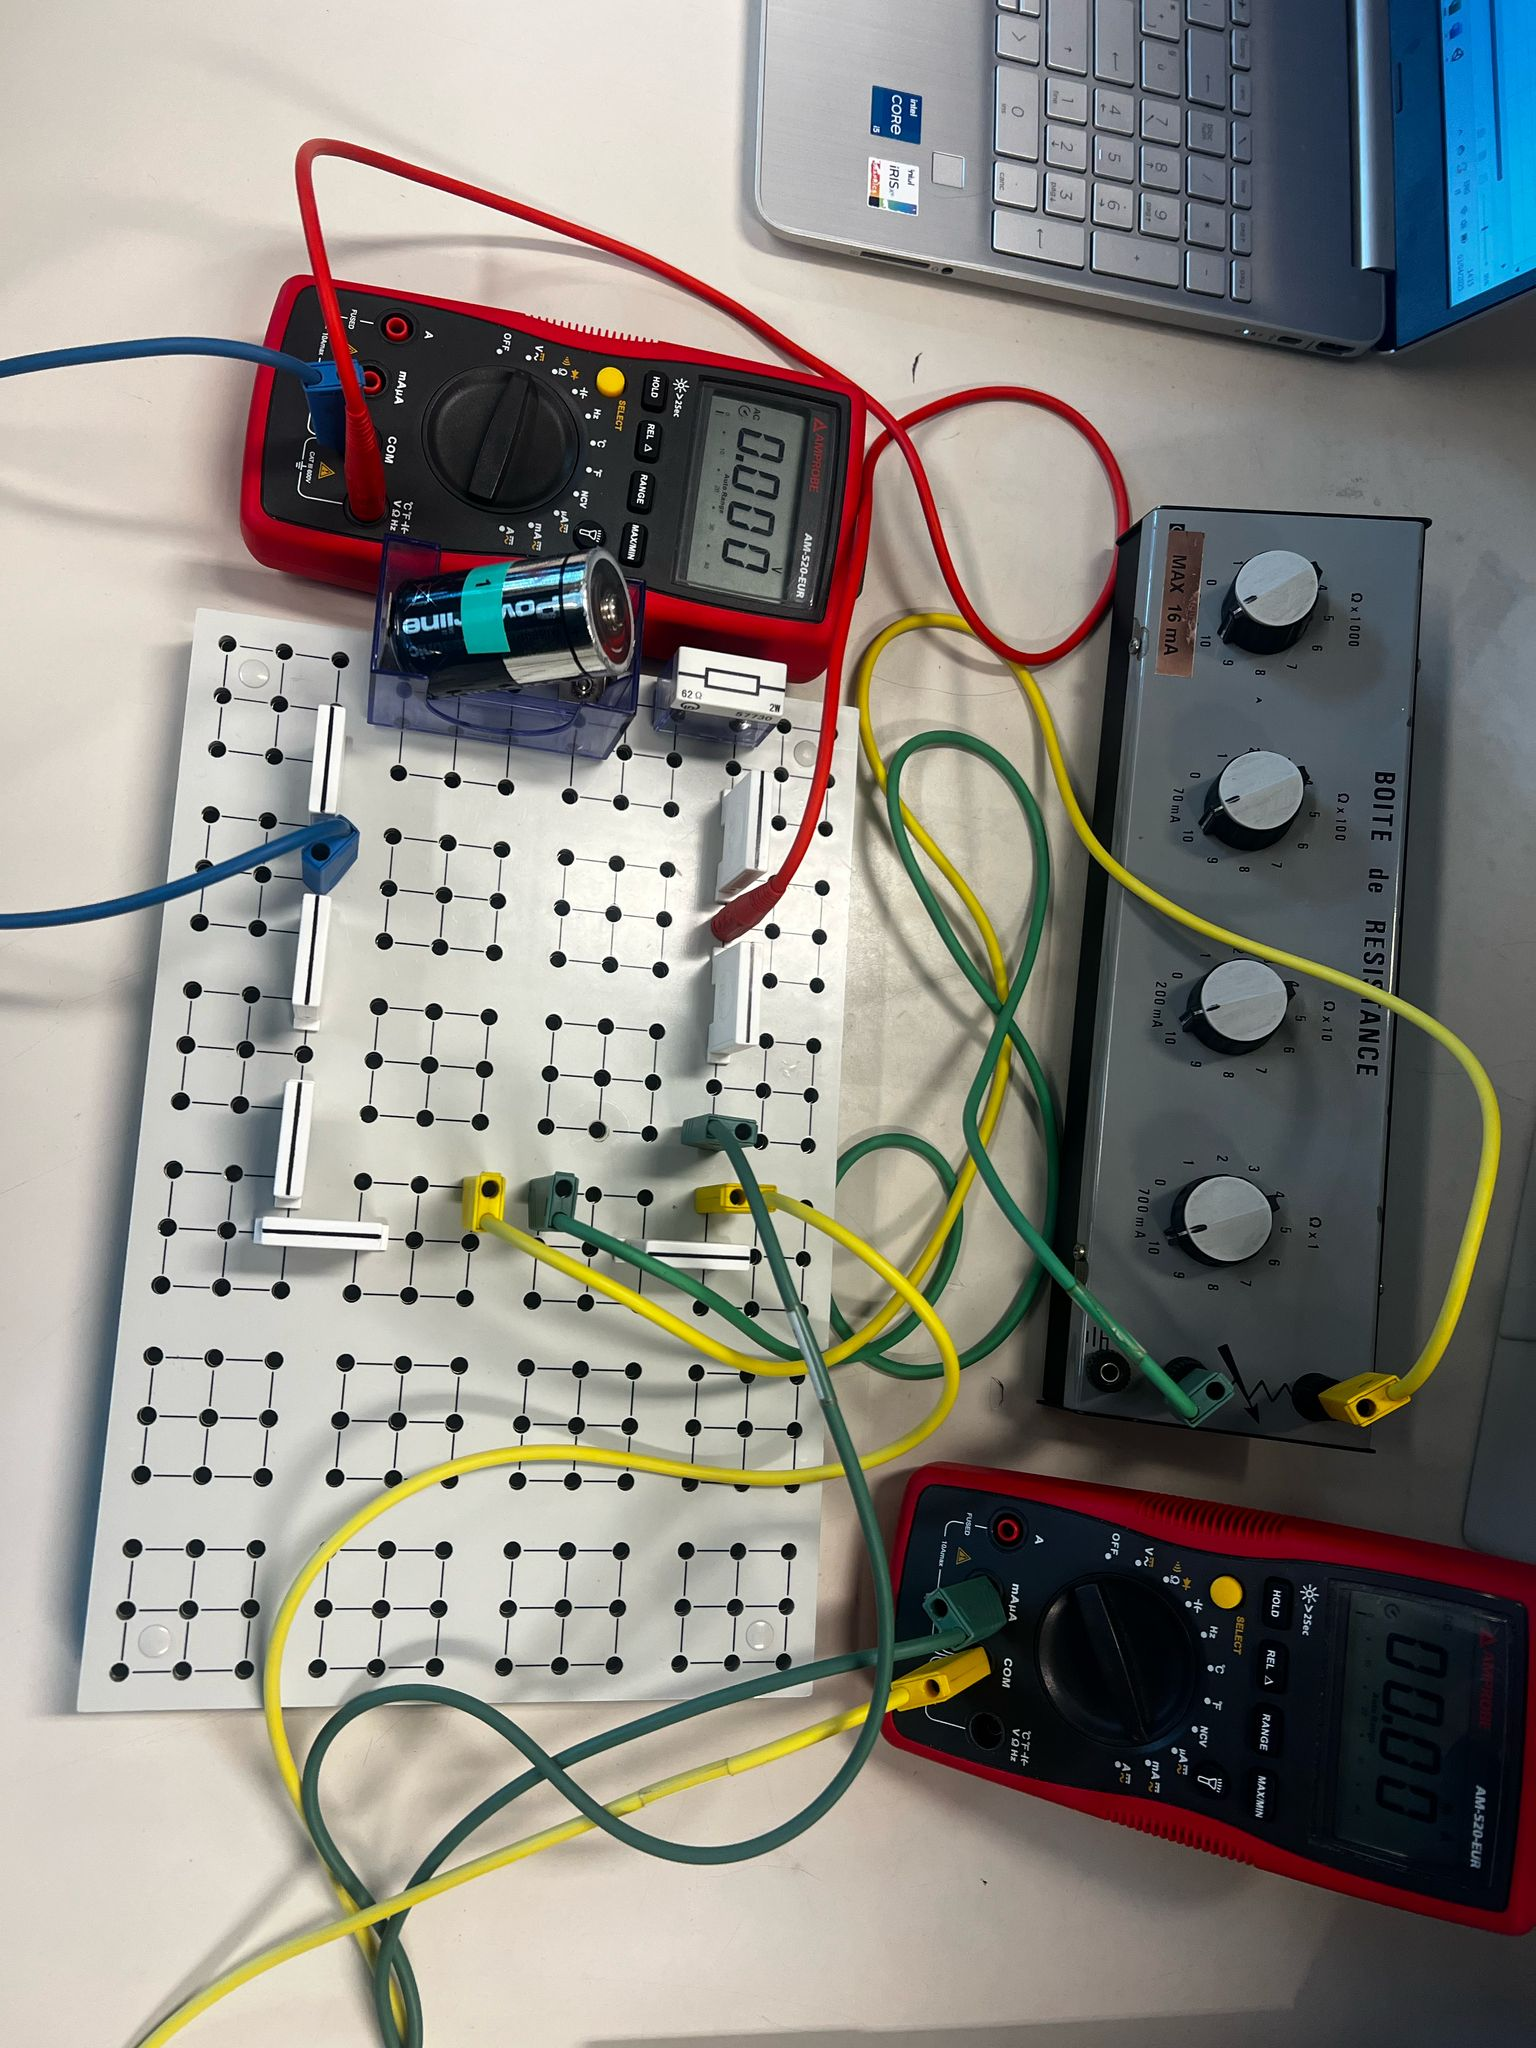
\includegraphics[width = 0.4\textwidth, angle = 90]{firstexp.jpeg}
    \label{fig:4}
    \caption{Experimental set-up for the first experiment}
\end{figure}


To measure the effect of combining multiple sources together, the same method
of measurement is used, whilst having the two different types of sources
connected, either in parallel, or in series. Figures 5(a) and 5(b) show the physical set-up of the combined source circuits.

\begin{figure}[!ht]
    \centering
    \begin{subfigure}{0.5\textwidth}
        \centering
        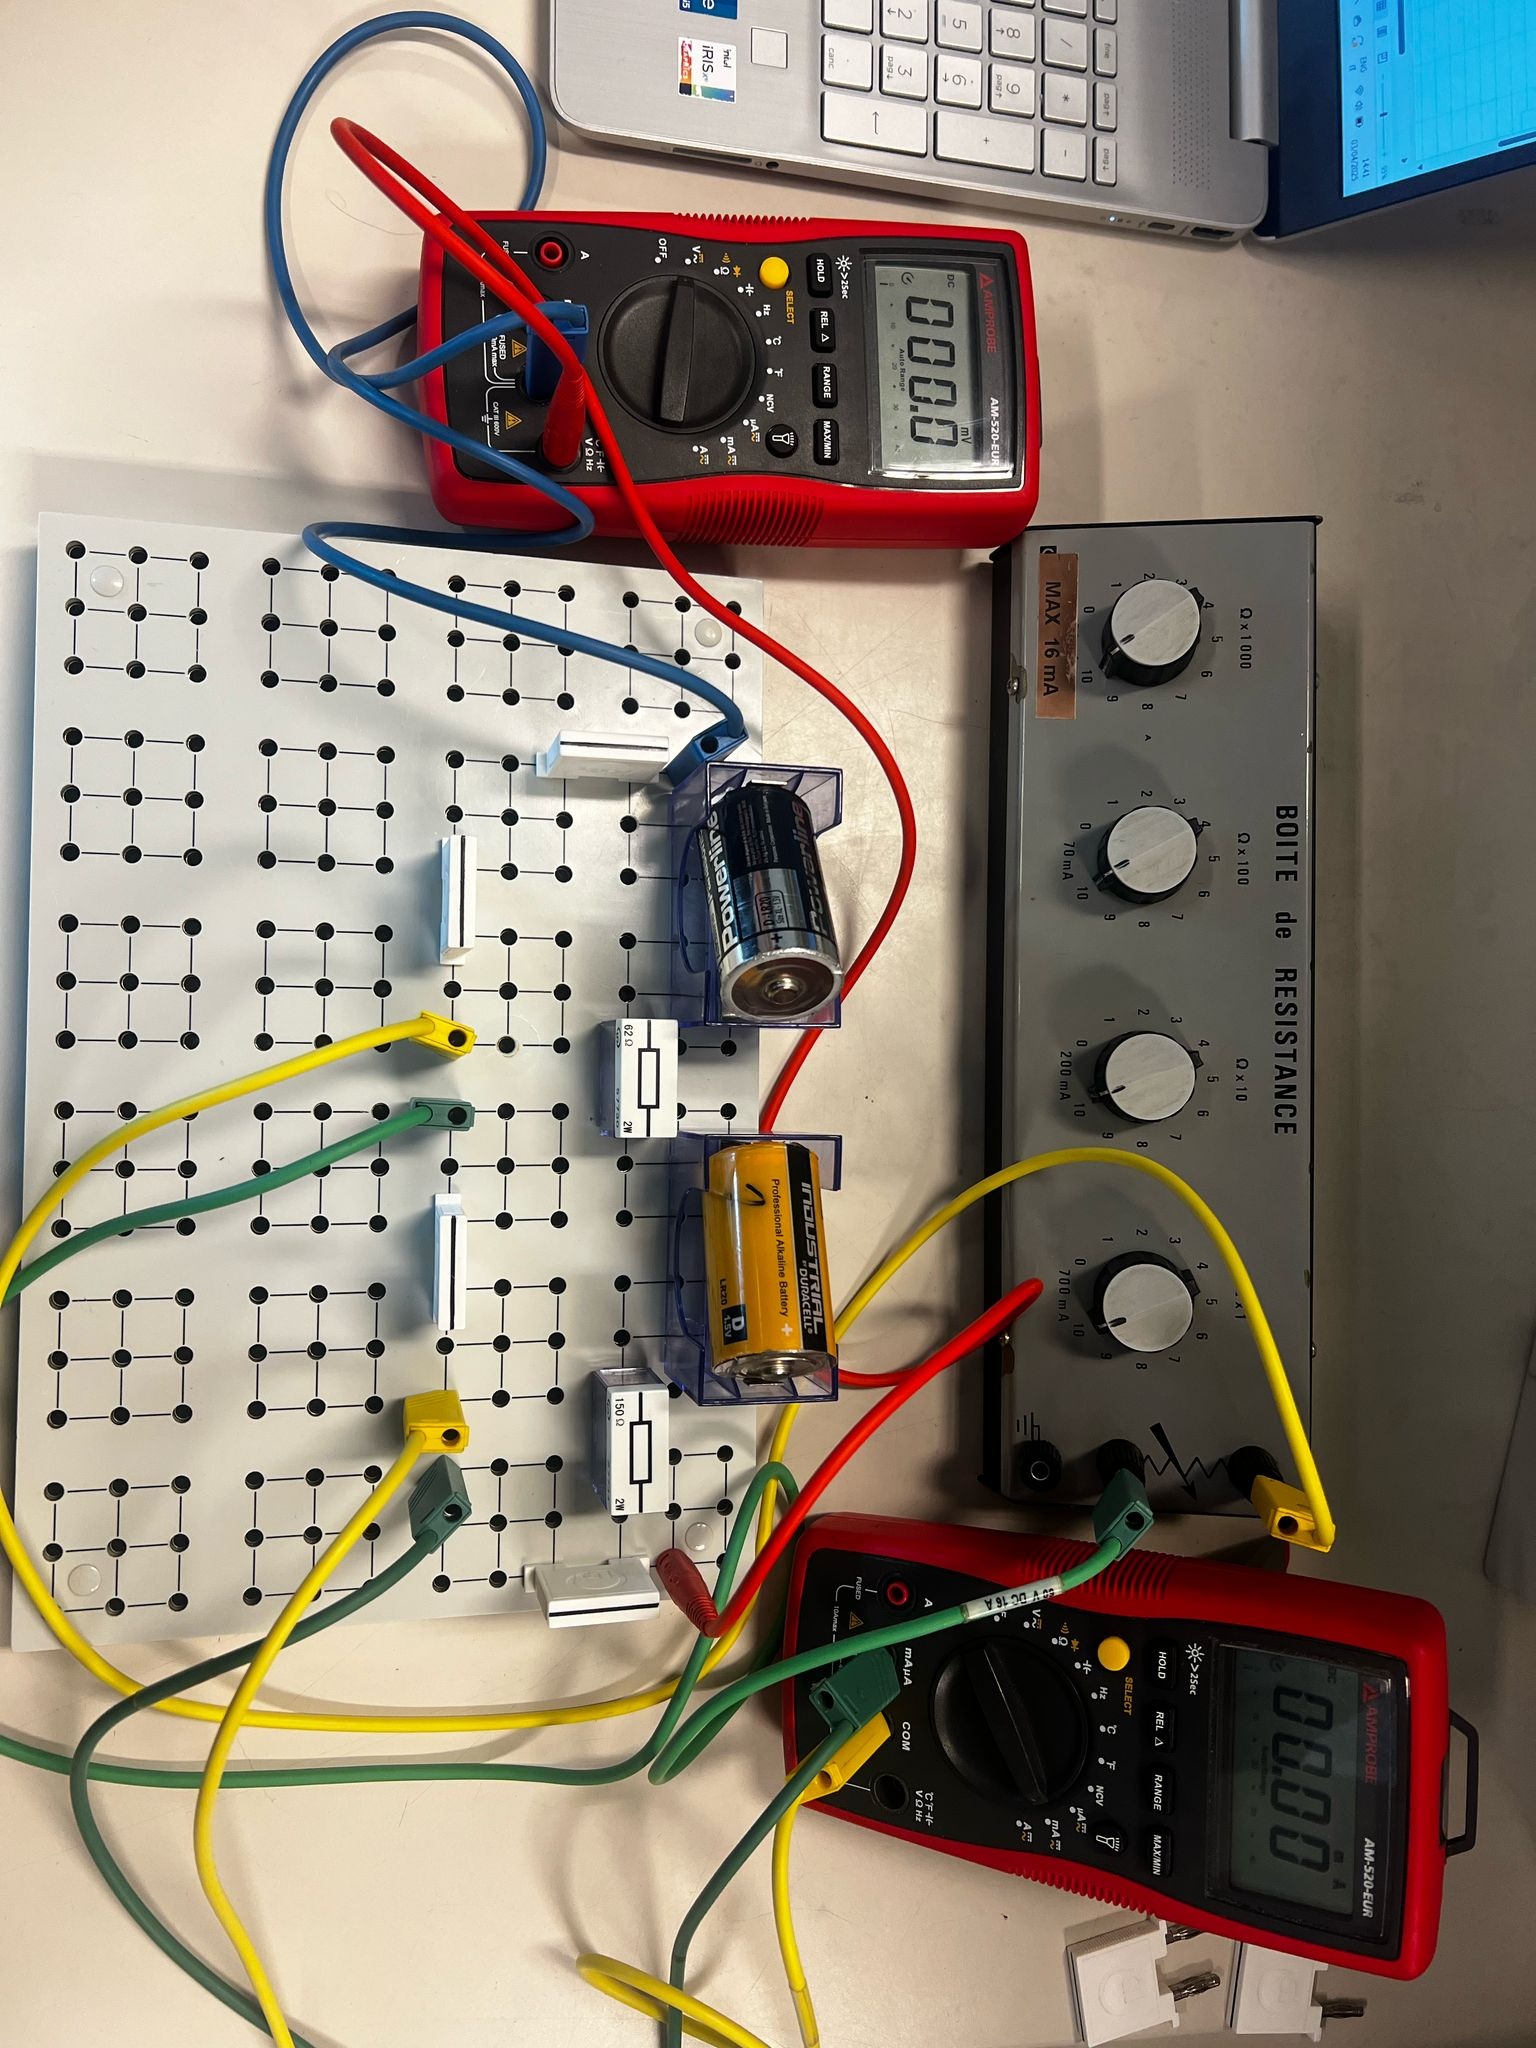
\includegraphics[width = 0.6\linewidth, angle = 90]{series.jpeg}
        \label{fig:5a}
        \caption{Series sources circuit}
    \end{subfigure}%
    \begin{subfigure}{0.5\textwidth}
        \centering
        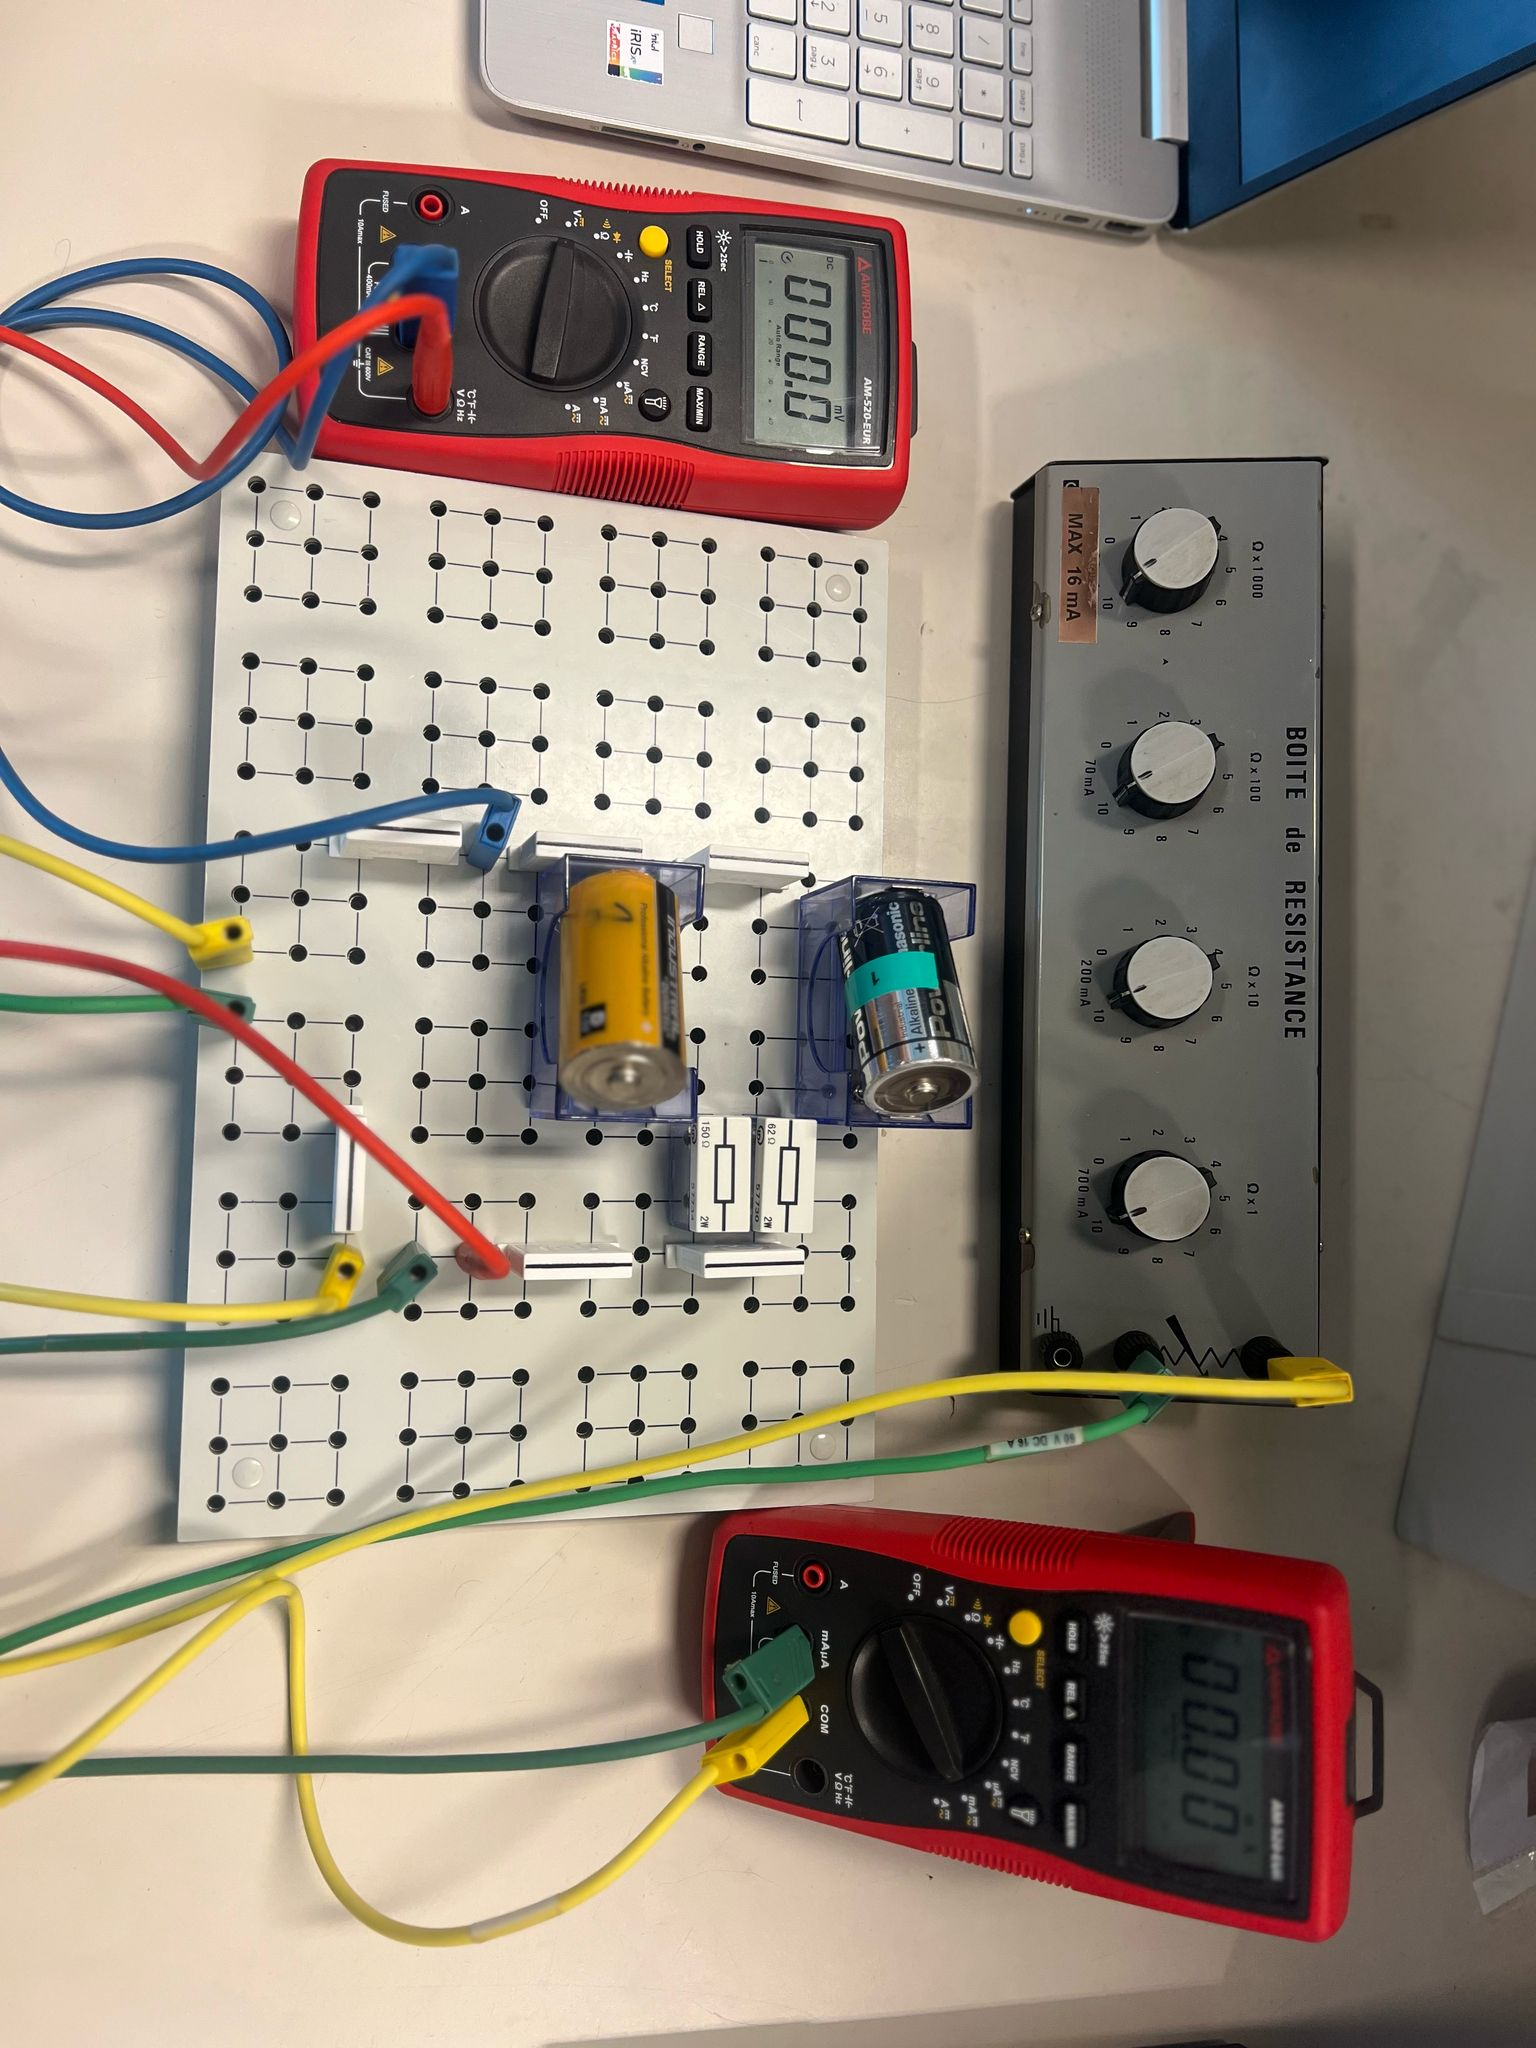
\includegraphics[width = 0.6\linewidth, angle = 90]{parallel.jpeg}
        \label{fig:5b}
        \caption{Parallel sources circuit}
    \end{subfigure}
    \label{fig:5}
    \caption{Experimental set-ups for the combined sources}
\end{figure}

\subsection{Experimental set-up maximum power transfer}
To determine the maximum power transfer, the same set-up as the last experiment
is used, without the ammeter. For source 1, the value of the load resistor is
varied between $30\unit{\Omega}$ and $120\unit{\Omega}$ in increments of 10,
whereas source 2, the value varies between $70\unit{\Omega}$ and
$250\unit{\Omega}$. The voltage across the load resistor is measured each time.
Additionally, the resistance of the decade resistor is measured after each
change.

\newpage
Figure 6 displays the physical set-up used to determine the maximum power
transfer of each source.

\begin{figure}[!ht]
    \centering
    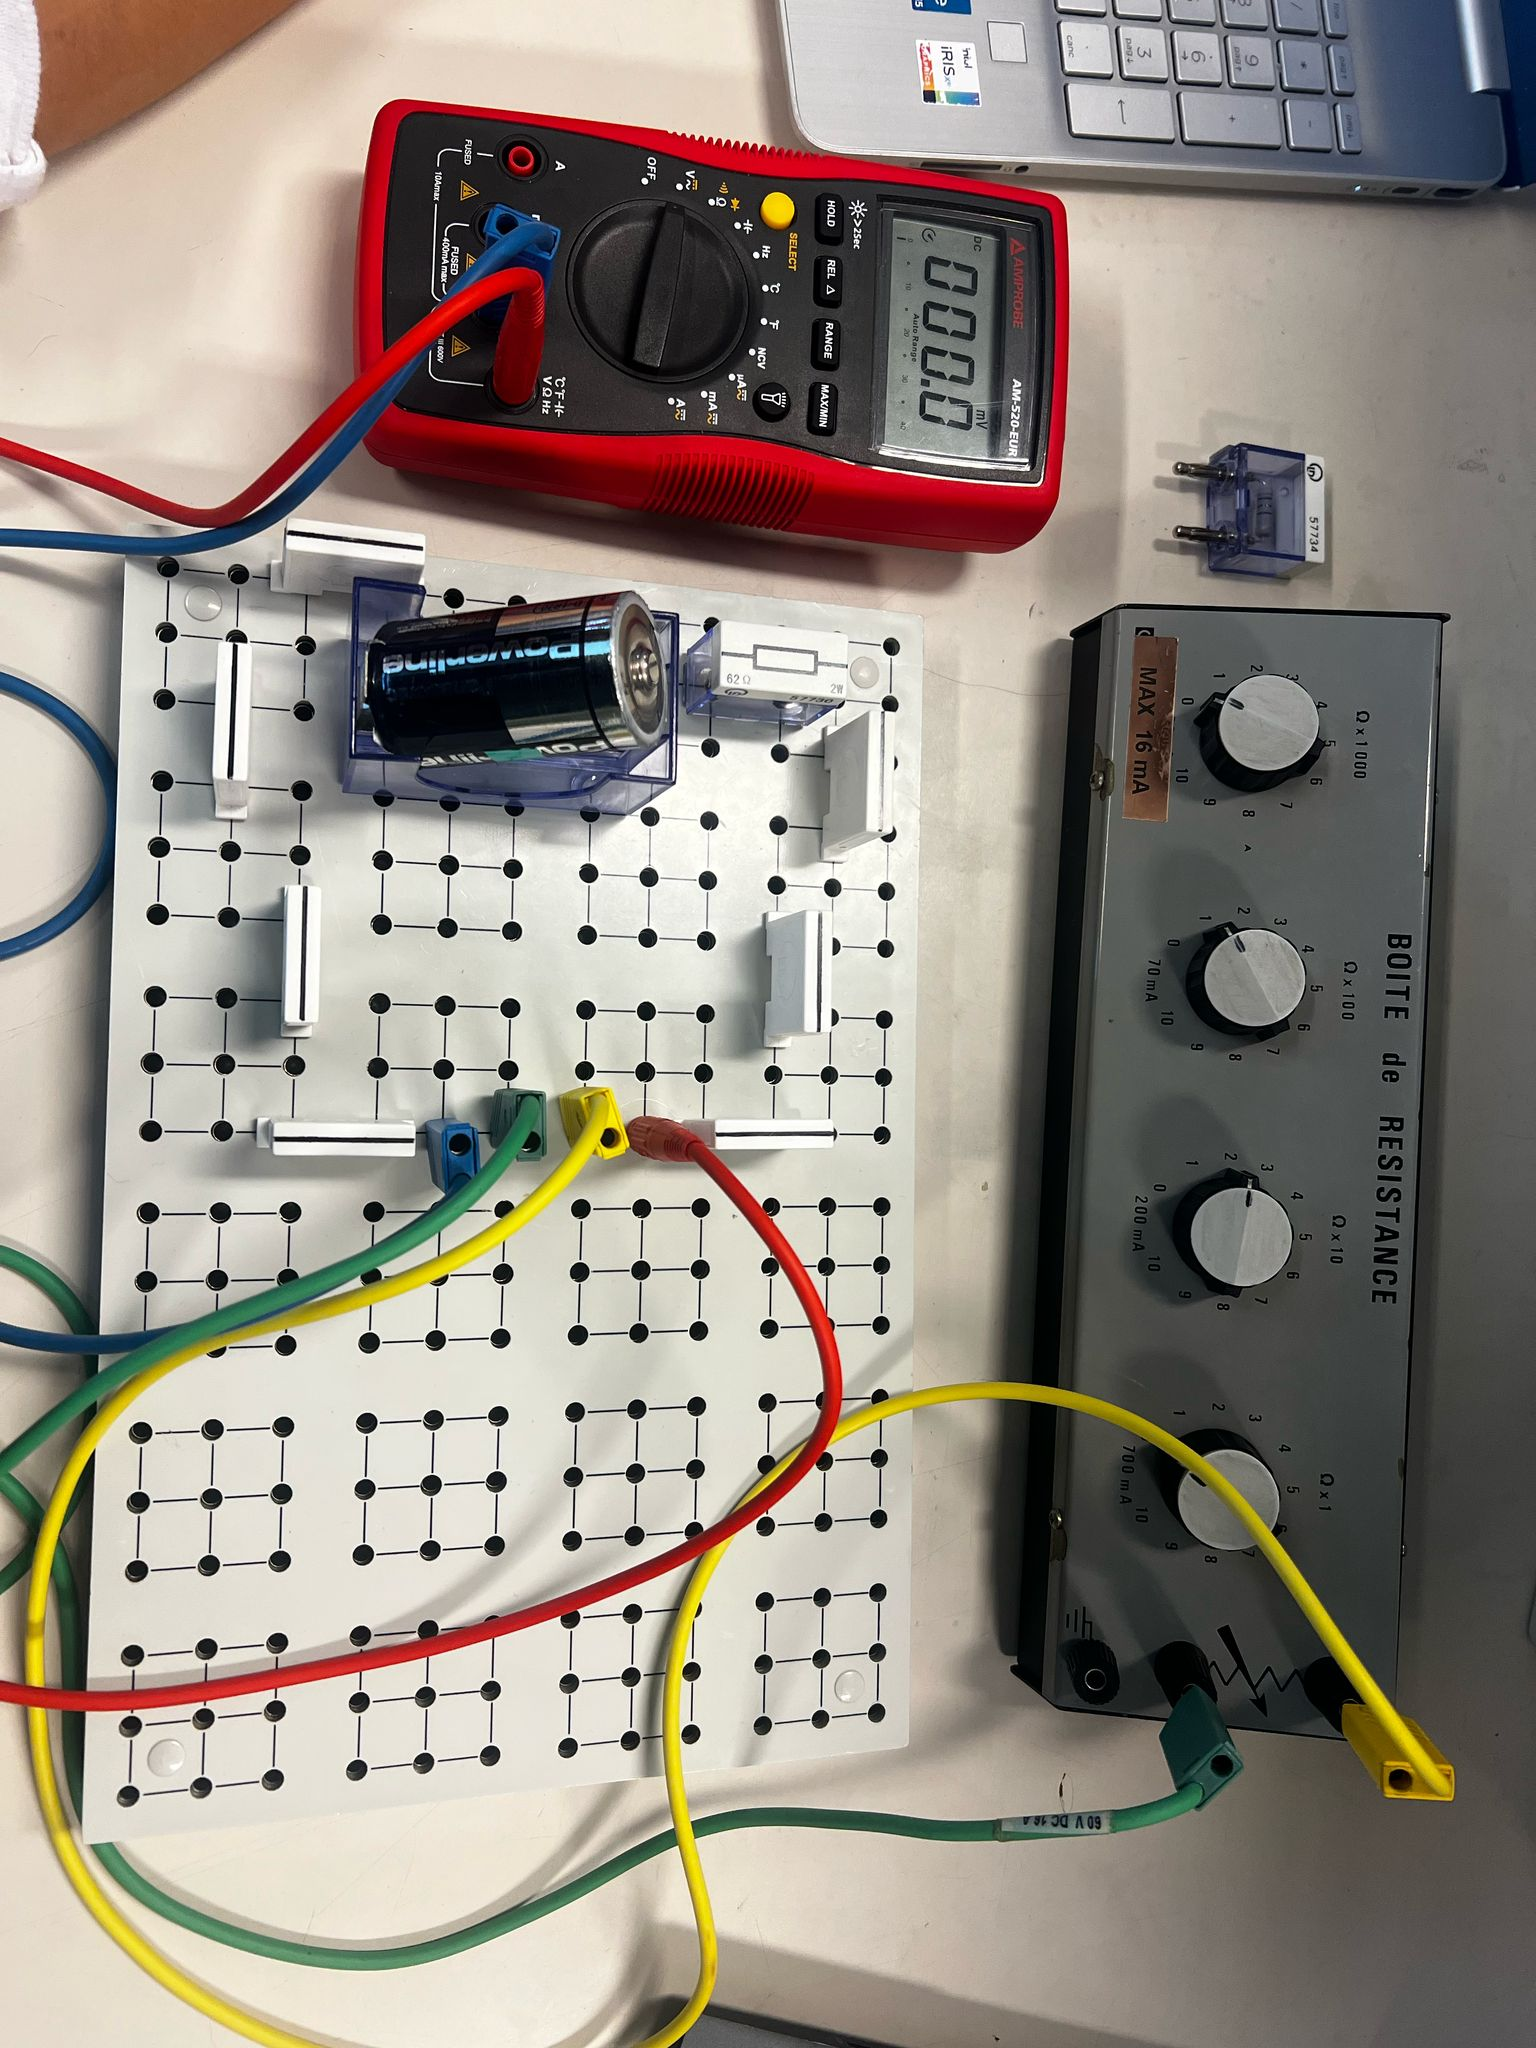
\includegraphics[width = 0.4\textwidth, angle = 90]{powertransf.jpeg}
    \label{fig:6}
    \caption{Experimental set-up of the power transfer experiment}    
\end{figure}

\newpage
\section{Determination of internal resistance}
\subsection{Measurement results}
After following the experimental flow as described in section 3.1, the determined
voltages are noted down. Afterwards the fixed resistors used as internal
resistances are measured using an ohmmeter. These are determined to be
$61.5\unit{\Omega}$ and $148.2\unit{\Omega}$ respectively. 

The measured load voltage of every source variation and the achieved load
current are displayed in Table 1.

\begin{table}[!ht]
    \centering
    \label{tab:1}
    \caption{Measurement results used to determine internal resistances}
    \begin{tabular}{ccccc} 
    \hline
    \makecell{$I_L$\\$\unit{(mA)}$} & \makecell{$V_{L_1}$\\$\unit{(V)}$} &
    \makecell{$V_{L_2}$\\$\unit{(V)}$} & \makecell{$V_{L_{ser}}$ \\ $\unit{(V)}$} &
    \makecell{$V_{L_{par}}$\\ $\unit{(V)}$}
    \\ 
    \hline
    0        & 1.49     & 1.49     & 3.004         & 1.496       \\
    0.5   & 1.459    & 1.415    & 2.897         & 1.475       \\
    1    & 1.429    & 1.342    & 2.793         & 1.453       \\
    1.5   & 1.398    & 1.268    & 2.687         & 1.431       \\
    2    & 1.367    & 1.193    & 2.584         & 1.409       \\
    2.5   & 1.336    & 1.121    & 2.48          & 1.388       \\
    3  & 1.305    & 1.047    & 2.375             & 1.366       \\
    3.5   & 1.275    & 0.974    & 2.271         & 1.344       \\
    4    & 1.244    & 0.899    & 2.168         & 1.322       \\
    4.5  & 1.213    & 0.827    & 2.063         & 1.3         \\
    5    & 1.183    & 0.752    & 1.959         & 1.279       \\
    \hline
    \end{tabular}
    \end{table}

\subsection{Graphs}
By plotting the load voltage in terms of $I_L$, all of a source's
characteristics can be determined. 

Figure 7 displays the relationship between load current and voltage for source
1, having an internal resistance of $61.5\unit{\Omega}$.


    \begin{figure}[!ht]
        \centering
        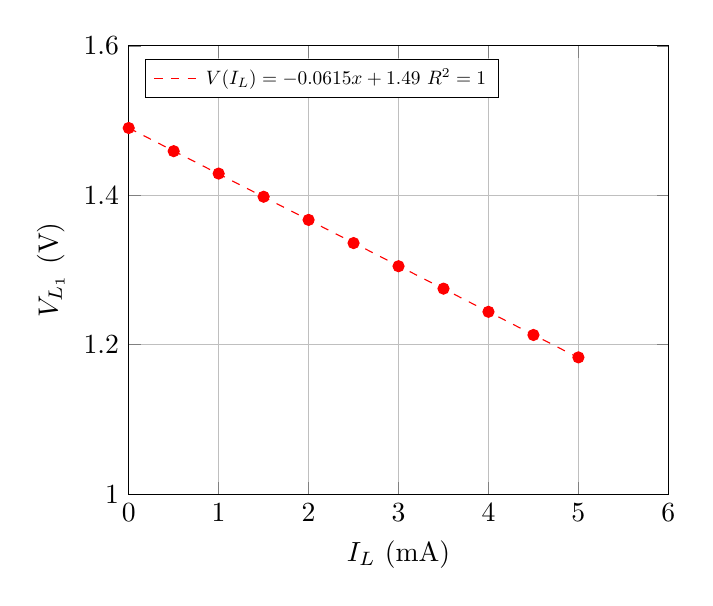
\begin{tikzpicture}
            \begin{axis}[
                xlabel = {$I_L\unit{(mA)}$},
                ylabel = {$V_{L_1}\unit{(V)}$},
                xmin = 0, xmax = 6,
                ymin = 1, ymax = 1.6,
                xtick = {0, 1, 2, 3, 4, 5, 6},
                ytick = {1, 1.2, 1.4, 1.6},
                ymajorgrids = true,
                xmajorgrids = true,
                legend pos = north west,
                legend style={nodes={scale=0.7}},
                domain = 0:5,
            ]
            
            \addplot[red, samples = 100, dashed]{-0.0615*x + 1.49};
            
            \addplot[only marks, color = red] coordinates {
                (0,	1.49)
                (0.5,	1.459)
                (1,	1.429)
                (1.5,	1.398)
                (2,	1.367)
                (2.5,	1.336)
                (3,	1.305)
                (3.5,	1.275)
                (4,	1.244)
                (4.5,	1.213)
                (5,	1.183)
                
            };
            
            \legend{$V(I_L) = -0.0615x + 1.49$ $R^2 = 1$}
            
            \end{axis}
        \end{tikzpicture}
        \caption{Load voltage of the first source in terms of load current}
        \label{fig:7}
    \end{figure}

\newpage
Figure 8 shows the relationship between $I_L$ and $V_{L_2}$, source 2 having an
internal resistance of $148.2\unit{\Omega}$

\begin{figure}[!ht]
    \centering
    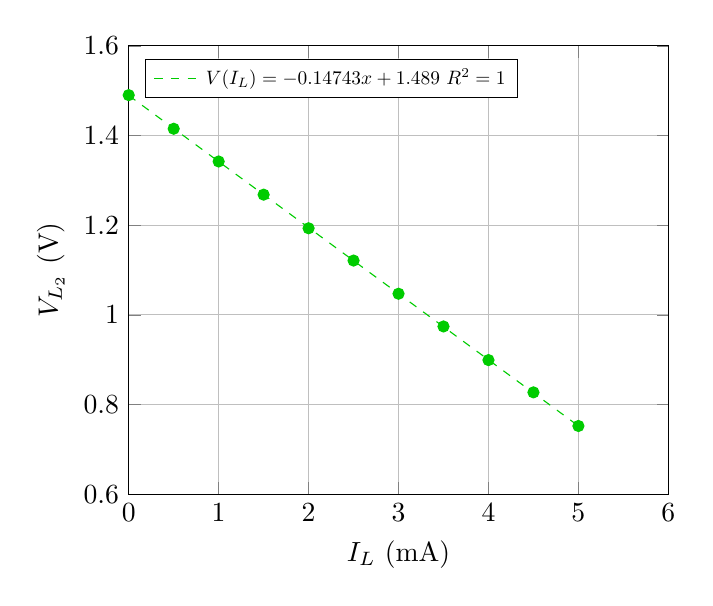
\begin{tikzpicture}
        \begin{axis}[
            xlabel = {$I_L\unit{(mA)}$},
            ylabel = {$V_{L_2}\unit{(V)}$},
            xmin = 0, xmax = 6,
            ymin = 0.6, ymax = 1.6,
            xtick = {0, 1, 2, 3, 4, 5, 6},
            ytick = {0.6, 0.8, 1, 1.2, 1.4, 1.6},
            ymajorgrids = true,
            xmajorgrids = true,
            legend pos = north west,
            legend style={nodes={scale=0.7}},
            domain = 0:5,
        ]
        
        \addplot[black!20!green, samples = 100, dashed]{-0.14743 * x + 1.4893};
        
        \addplot[only marks, color = black!20!green] coordinates {
            (0,	1.49)
            (0.5,	1.415)
            (1,	1.342)
            (1.5,	1.268)
            (2,	1.193)
            (2.5,	1.121)
            (3,	1.047)
            (3.5,	0.974)
            (4,	0.899)
            (4.5,	0.827)
            (5,	0.7520)
        };
        
        \legend{$V(I_L) = -0.14743x + 1.489$ $R^2 = 1$}
        
        \end{axis}
    \end{tikzpicture}
    \caption{Load voltage of the second source in terms of load current}
    \label{fig:8}
\end{figure}

Figure 9 displays the voltage current dependency for the series source
arrangement.

\begin{figure}[!ht]
    \centering
    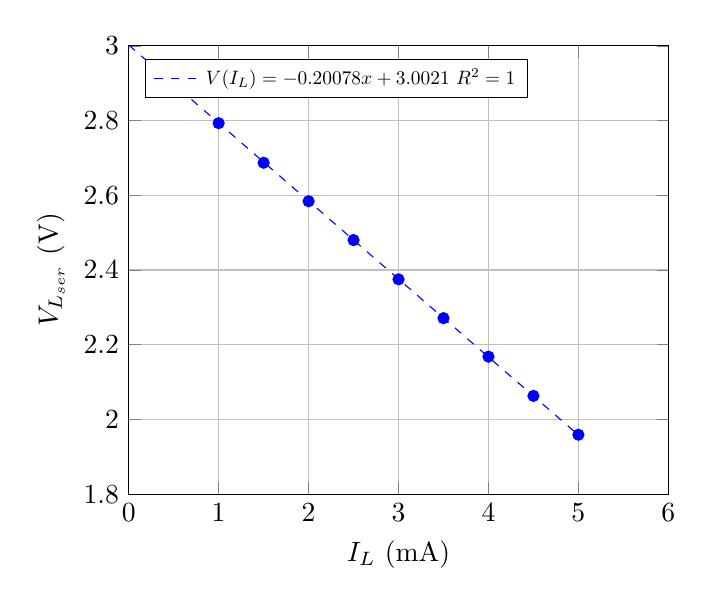
\begin{tikzpicture}
        \begin{axis}[
            xlabel = {$I_L\unit{(mA)}$},
            ylabel = {$V_{L_{ser}}\unit{(V)}$},
            xmin = 0, xmax = 6,
            ymin = 1.8, ymax = 3,
            xtick = {0, 1, 2, 3, 4, 5, 6},
            ytick = {1.8, 2, 2.2, 2.4, 2.6, 2.8, 3},
            ymajorgrids = true,
            xmajorgrids = true,
            legend pos = north west,
            legend style={nodes={scale=0.7}},
            domain = 0:5,
        ]
        
        \addplot[blue, samples = 100, dashed]{-0.20878 * x + 3.0021};
        
        \addplot[only marks, color = blue] coordinates {
            (0,	3.004)
            (0.5,	2.897)
            (1,	2.793)
            (1.5,	2.687)
            (2,	2.584)
            (2.5,	2.48)
            (3,	2.375)
            (3.5,	2.271)
            (4,	2.168)
            (4.5,	2.063)
            (5,	1.959)
            
        };
        
        \legend{$V(I_L) = -0.20078x + 3.0021$ $R^2 = 1$}
        
        \end{axis}
    \end{tikzpicture}
    \caption{Load voltage of the series source arrangement in terms of load current}
    \label{fig:9}
\end{figure}

\newpage
Figure 10 represents the linear relationship between load current and load
voltage for the parallel source arrangements.

\begin{figure}[!ht]
    \centering
    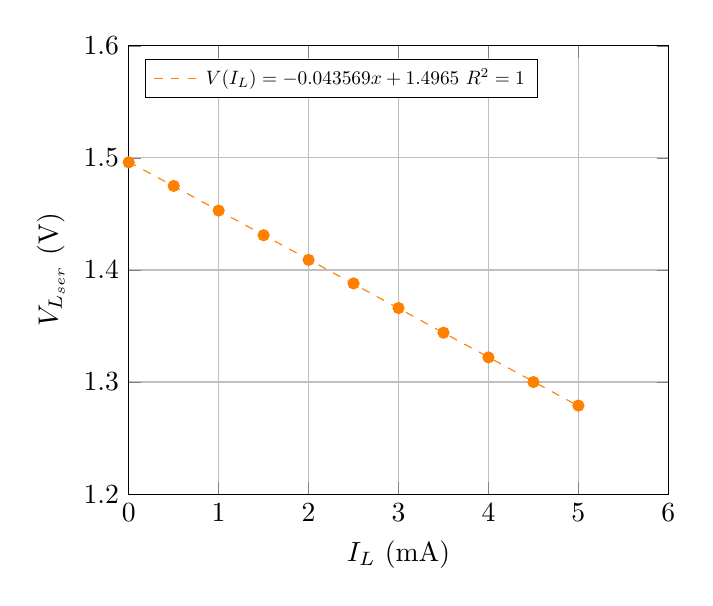
\begin{tikzpicture}
        \begin{axis}[
            xlabel = {$I_L\unit{(mA)}$},
            ylabel = {$V_{L_{ser}}\unit{(V)}$},
            xmin = 0, xmax = 6,
            ymin = 1.2, ymax = 1.6,
            xtick = {0, 1, 2, 3, 4, 5, 6},
            ytick = {1.2, 1.3, 1.4, 1.5, 1.6},
            ymajorgrids = true,
            xmajorgrids = true,
            legend pos = north west,
            legend style={nodes={scale=0.7}},
            domain = 0:5,
        ]
        
        \addplot[orange, samples = 100, dashed]{-0.043569 * x + 1.4965};
        
        \addplot[only marks, color = orange] coordinates {
            (0,	1.496)
            (0.5,	1.475)
            (1,	1.453)
            (1.5,	1.431)
            (2,	1.409)
            (2.5,	1.388)
            (3,	1.366)
            (3.5,	1.344)
            (4,	1.322)
            (4.5,	1.3)
            (5,	1.279)
            
        };
        
        \legend{$V(I_L) = -0.043569x + 1.4965$ $R^2 = 1$}
        
        \end{axis}
    \end{tikzpicture}
    \caption{Load voltage of the parallel source arrangement in terms of load current}
    \label{fig:10}
\end{figure}
\subsection{Calculations}
By utilizing the equations described in section 2.1, the characteristics of both
sources can be determined. 

The result of these calculations is displayed in table 2.


\begin{table}[!ht]
    \centering
    \label{tab:2}
    \caption{Calculated source characteristics}
    \begin{tabular}{cccc} 
    \hline
    Source  & \makecell{$R_i$\\ $\unit{\Omega}$}     & \makecell{$V_{emf}$\\$\unit{V}$}  & \makecell{$I_{sc}$\\$\unit{mA}$}         \\ 
    \hline
    Source 1 & 61.5   & 1.49  & 24.22  \\
    Source 2 & 147.4 & 1.49  & 10.11  \\
    Series  & 208.8 & 3     & 14.37  \\
    Parallel & 43.6 & 1.49 & 34.34  \\
    \hline
    \end{tabular}
    \end{table}

To determine the error of the internal resistance measurements, Microsoft
Excel's LINEST function is used. This function returns information about linear
regression of a set of samples. One of these values is the standard error for
$V_{L}$. It is important to mention that all the error values will be rounded
up to one significant figure, as instructed in the uncertainty analysis manual(unc). This value can be used to calculate the error of the internal
resistance. This is done by using equation 5. This will also be used to determine the
error of $I_{sc}$. 

\begin{equation}
    \Delta R_i = R_i \frac{\Delta V}{V}
\end{equation}

Therefore, the following calculations are made:
\begin{gather*}
    \Delta R_i = 61.5 \frac{6.5 \cdot 10^{-5}}{1.183} \approx 0.1\unit{\Omega}\\
    \Delta I_{sc} = 21.22 \frac{6.5\cdot 10^-5}{1.183} \approx 0.01\unit{mA}
\end{gather*}

Therefore the values of $R_i$ and $I_{sc}$ for source one are:
\begin{gather*}
    R_i = (61.5\pm 0.1)\unit{\Omega}\\
    I_{sc} = (21.22 \pm 0.01)\unit{mA}
\end{gather*}

However, the error of $V_{emf}$ will be determined using the error of the
multimeter measurements(mm). This is done using equation 6.
\begin{equation}
    \Delta V_{emf} = \frac{V}{100} + 3 LSD
\end{equation}

By introducing the measured value for source one, the following calculation is
achieved:

\[ \Delta V_{emf} = \frac{1.49}{100} + 0.003 \approx 0.02 \unit{V}\]

Therefore, the value for electromotive force is:
\[V_{emf} = (1.49 \pm 0.02)\unit{V}\]

The error of the internal resistance fixed resistors will also be determined by
using the error of the multimeter. The formula used is shown in equation 7.

\begin{equation}
    \Delta R = \frac{1.2 \cdot R}{100} + 2LSD
\end{equation}

The sample calculation for the internal resistance of the first source, $R_{i_1}$, is:

\[\Delta R_{i_1} = \frac{1.2 \cdot 61.5}{100} + 0.002 \approx 0.8\unit{\Omega}\]

Therefore, the values of the measured internal resistances are:
\begin{gather*}
    R_{i_1} = (61.5 \pm 0.8)\unit{\Omega}\\
    R_{i_2} = (148.2 \pm 2)\unit{\Omega}
\end{gather*}

\subsection{Discussion}
The determination of internal resistance for the two different voltage sources
and their respective arrangements proved to be accurate. By comparing the
measured values, using an ohmmeter, to the calculated values, one can observe
that the calculations produce results which fall in the range of the
measurements \textemdash $R_{i_2,c} = (147.4 \pm 0.1)\unit{\Omega}$ - $R_{i_2,m}
= (148.2 \pm 2)\unit{\Omega}$. Therefore, this mode of measurement proves to be
accurate.

By analyzing the behaviour of the two source arrangements, it is observed that
these adhere to the exactly to the mechanisms described in Section 2.2. The
increase of both electromotive force and internal resistance is present in the
series source configuration. Additionally, a decrease of the internal resistance
is seen when the two sources are connected in parallel, while $V_{emf}$ remains
the same.

While it may seem tempting to determine the real internal resistance of the
battery by using these measurements, it is not possible, as alkaline batteries
have an internal resistance of around $0.5 \unit{\Omega}$ at room temperature
(battery). This value is smaller than the error of the ohmmeter when measuring
the resistance of the fixed resistors. Therefore, we cannot conclude how much of
a role the real internal resistance played.

\newpage
\section{Maximum power transfer}
\subsection{Measurement results}
After following the experimental flow as described in section 3.2, the measured
values for $R_L$ and $V_L$ are noted down. Afterwards the necessary calculations
are done to determine the value of $P_L$. This is done for both sources. For
source 1 the results are displayed in Table 3.
\begin{table}[!ht]
    \centering
    \label{tab:3}
    \caption{Power transfer results for source 1}
    \begin{tabular}{cccc} 
    \hline
    \makecell{$R_L$\\$\unit{(\Omega)}$} & \makecell{$R_m$\\$\unit{(\Omega)}$} & \makecell{$V_l$\\$\unit{(V)}$}  & \makecell{$P_l$\\$\unit{(mW)}$}     \\ 
    \hline
    30   & 30.2        & 0.487 & 7.85  \\
    40   & 40.2        & 0.585 & 8.51   \\
    50   & 50.2        & 0.666 & 8.84  \\
    60   & 60.2        & 0.733 & 8.93  \\
    70   & 70.2        & 0.79  & 8.89  \\
    80   & 80.2        & 0.839 & 8.78  \\
    90   & 90.2        & 0.882 & 8.62  \\
    100  & 100.3       & 0.918 & 8.40   \\
    110  & 109.9       & 0.951 & 8.23  \\
    120  & 119.9       & 0.981 & 8.03  \\
    \hline
    \end{tabular}
    \end{table}

Table 4 displays the resulting values for the second source. However, it is
important to mention that since the third data point does not follow the
expected behaviour, it will be considered an outlier.

\begin{table}[!ht]
    \centering
    \label{tab:4}
    \caption{Power transfer results for source 2}
    \begin{tabular}{cccc} 
    \hline
    \makecell{$R_L$\\$\unit{(\Omega)}$} & \makecell{$R_m$\\$\unit{(\Omega)}$} & \makecell{$V_l$\\$\unit{(V)}$}  & \makecell{$P_l$\\$\unit{(mW)}$}     \\
    \hline
    70  & 70.2  & 0.477 & 3.24  \\
    90  & 90.2  & 0.562 & 3.50  \\
    \tikzmark{start} 110 & 109.8 & 0.33  & 0.99 \tikzmark{end}  \\
    130 & 129.8 & 0.694 & 3.71  \\
    150 & 149.9 & 0.747 & 3.72  \\
    170 & 169.9 & 0.793 & 3.70  \\
    190 & 190   & 0.835 & 3.67  \\
    210 & 201.1 & 0.855 & 3.64  \\
    230 & 221.2 & 0.89  & 3.58  \\
    250 & 241.2 & 0.92  & 3.51  \\
    \hline
    \end{tabular}
    \tikz[remember picture] \draw[overlay] ([yshift=.35em]pic cs:start) -- ([yshift=.35em]pic cs:end);
    \end{table}
\newpage
\subsection{Graphs}
By plotting the power dissipated on the load resistor as a function of the load
resistance, the maximum power transfer can be easily seen. However, since the
resistance is incremented in steps of $10\unit{\Omega}$, the maximal transfer
will not be precisely determined. Figure 11 shows the relationship between $P_L$
and $R_L$.

\begin{figure}[!ht]
    \centering
    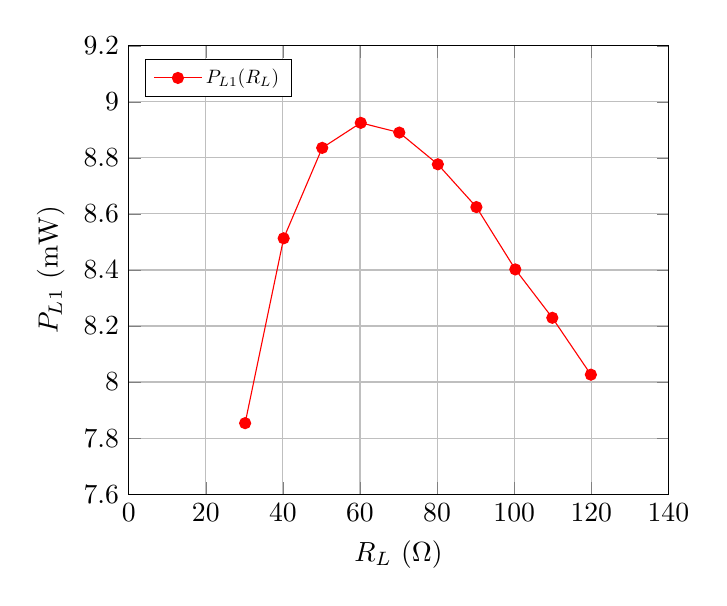
\begin{tikzpicture}
        \begin{axis}[
            xlabel = {$R_L\unit{(\Omega)}$},
            ylabel = {$P_{L1}\unit{(mW)}$},
            xmin = 0, xmax = 140,
            ymin = 7.6, ymax = 9.2,
            xtick = {0, 20, 40, 60, 80, 100, 120, 140},
            ytick = {7.6, 7.8, 8, 8.2, 8.4, 8.6, 8.8, 9, 9.2},
            ymajorgrids = true,
            xmajorgrids = true,
            legend pos = north west,
            legend style={nodes={scale=0.7}},
            domain = 0:5,
        ]
        
        \addplot[mark = *, color = red] coordinates {
            (30.2,	7.853278146)
            (40.2,	8.513059701)
            (50.2,	8.835776892)
            (60.2,	8.925066445)
            (70.2,	8.89031339)
            (80.2,	8.777069825)
            (90.2,	8.62443459)
            (100.3,	8.402033898)
            (109.9,	8.229308462)
            (119.9,	8.026363636)
            
        };
        
        \legend{$P_{L1}(R_L)$}
        
        \end{axis}
    \end{tikzpicture}
    \caption{Power in terms of load resistance for the first source}
    \label{fig:11}
\end{figure}

The same graph can also be made for the second source, this is shown in figure
12.

\begin{figure}[!ht]
    \centering
    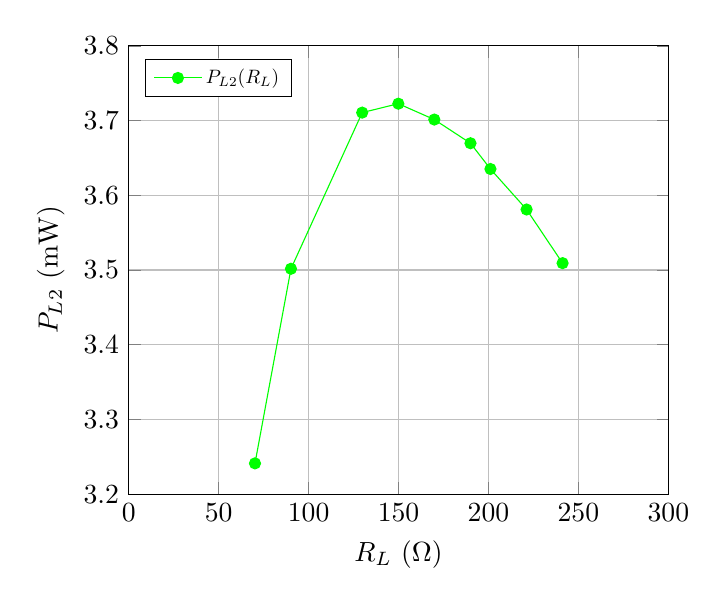
\begin{tikzpicture}
        \begin{axis}[
            xlabel = {$R_L\unit{(\Omega)}$},
            ylabel = {$P_{L2}\unit{(mW)}$},
            xmin = 0, xmax = 300,
            ymin = 3.2, ymax = 3.8,
            xtick = {0, 50, 100, 150, 200, 250, 300},
            ytick = {3.2, 3.3, 3.4, 3.5, 3.6, 3.7, 3.8},
            ymajorgrids = true,
            xmajorgrids = true,
            legend pos = north west,
            legend style={nodes={scale=0.7}},
            domain = 0:5,
        ]
        
        \addplot[mark = *, color = green] coordinates {
            (70.2,	3.241153846)
            (90.2,	3.501596452)
            (129.8,	3.710600924)
            (149.9,	3.722541694)
            (169.9,	3.701288994)
            (190,	3.669605263)
            (201.1,	3.635131775)
            (221.2,	3.580922242)
            (241.2,	3.509121061)
            
        };
        
        \legend{$P_{L2}(R_L)$}
        \end{axis}
    \end{tikzpicture}
    \caption{Power in terms of load resistance for the second source}
    \label{fig:12}
\end{figure}
\subsection{Calculations}
To determine the error of the maximum power dissipation for the first source,
the following error propagation formula has to be used:

\begin{equation}
    \Delta P_L = P_L\sqrt{\left(\frac{\Delta R_L}{R_L}\right) ^2 + \left( \frac{\Delta V_L}{V_L}\right) ^2}
\end{equation}

\newpage
Thus, both the error of $V_L$ and $R_L$ have to be determined. This will be done
by using equation 8 and 9, respectively. The calculation for $V_L$, using
equation 8, is:

\[\Delta V_L = \frac{0.733}{100} + 0.003 \approx 0.008 \unit{V}\]

Using equation 9, the calculation for $R_L$ can be made:
\[\Delta R_L = \frac{1.2\cdot 60.2}{100} + 0.4 \approx 2\unit{\Omega}\]

Finally, equation 10 can be used to determine the error of the maximum power
measurement:
\[\Delta P_L = 8.93\cdot \sqrt{\left(\frac{2}{60.2}\right ) ^2 + \left(
\frac{0.008}{0.768} \right) ^2} \approx 0.40\unit{mW}\]

Therefore, the maximum power dissipation for the first source is:

\[P_{max} = (8.93 \pm 0.40)\unit{mW}\]

\subsection{Discussion}

\end{document}